\subsubsection{Initial comparison - Default settings \label{sec:initialCompare}}
For the initial comparison we use the Bertsekas featureset, since the same featureset
was used for verifying the Cross Entropy implementation. Furthermore, others researchers
has used the Bertsekas featureset as a benchmarking standpoint \citep{thiery:09} \&
\citep{szita:06}.\\
The goal of this comparison is to get an initial idea of how the Shark implementation of
CMA-ES compares to Cross Entropy with settings used by other researchers \citep{thiery:09}.\\

\textbf{Results}

Using Cross Entropy with the constant noise setting and CMA with an initial step-size
of $0.5$, we get the following results, seen in figure \ref{fig:CMA_VS_CE_00}.\\

\begin{figure}[H]
\begin{center}
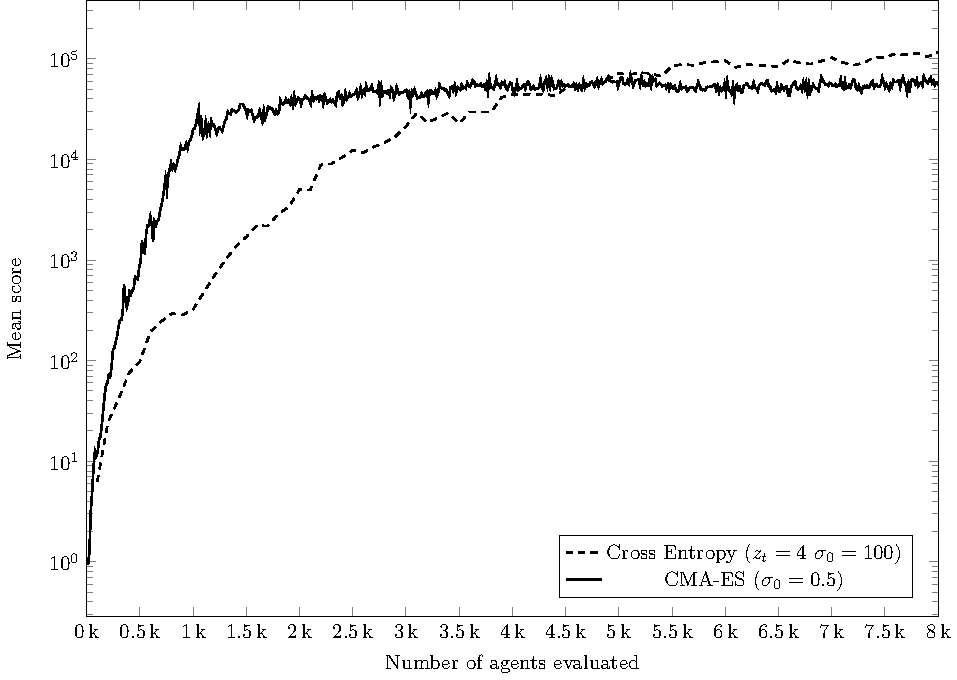
\includegraphics[scale=0.8]{plots/cmaCePlot}
\end{center}
\caption{Initial comparison between CMA-ES and Cross Entropy \label{fig:CMA_VS_CE_00}}
\end{figure}

\begin{table}[H]
\centering
\small
\begin{tabular}{l r r r r}
Optimizer & Mean & Q1 & Q2 & Q3\\
\hline
CMA-ES  & $57783.0$ & $10269.9$ & $59774.5$ & $100384.1$\\
Cross-entropy method & $116289.4$ & $85230.9$ & $125329.5$ & $138715.5$\\
\end{tabular}
\caption{Results from last iteration of the curves in figure \ref{fig:CMA_VS_CE_00}
\label{table:initialResultTable}}
\end{table}

As figure \ref{fig:CMA_VS_CE_00} reveals that CMA-ES converges faster,
but reaches a local optimum at around 2,000 games played. Meanwhile Cross Entropy has a 
slower convergence but reaches a better mean score compared to CMA-ES at around 5,500
agents evaluated. In detail, CMA-ES on average reaches a score of 50,000 rows, and
Cross Entropy reaches a score of 100,000.\\

\textbf{Analysis and discussion}

These results clearly defy our initial hypothesis as we predicted
for CMA-ES to outperform Cross-entropy method, due to its more sophisticated nature. 
One reason for this outcome could possibly be that
CMA-ES has a very little population size compared to Cross Entropy,
which could be a decisive lack as the objective function is noisy with 
a high variance.\\

\begin{changebar}
To perform a comparison between the two algorithms on the same terms,
we saw from earlier experiments that both algorithms benefits from 
adjusted settings. Thus, another experiment is required, where both algorithms
are adjust to have the best possible settings to ensure that both algorithms
perform as well as possible. Among the adjusted parameters are the following.\\
\\
\textit{Enlargment of population size}\\
Our first experiment clearly shows that the CMA-ES
is outperformed by the Cross-entropy method.
The CMa-ES does by default only have a relatively small
population size (around 13) compared to the Cross-entropy methods
default (100). From the earlier experiments, we saw that 
the Cross-entropy method does benefit from a higher populations size,
and to CMA-ES, the higher population size appears critical
to it's performance. Thus, the population size is increased for 
both algorithm in our final experiment.\\
\\
\textit{Evaluate each agent multiple times}\\
From our experiments, the Cross-entropy method does not
seem to require evaluation each search point more than once
and thus, the number of evaluations remains at 1 per
search point. For the CMA-ES however, with a 
ranking mechanism that strongly emphasizes 
the best search points in a population, a firm
ranking is important. Our experiments suggested that
evaluation each search point 5 times appears to be optimal 
for the CMA-ES.\\
\\
\textit{Change the recombination type}\\
As described in section \ref{CMAtheory}, 
the CMA-ES is not bound to update its 
new mean to just the centroid of the selected 
vectors. Instead, it can weight better solutions
more heavily when moving its mean. When doing so,
it risks biasing search points that appear to be better 
but in reality, just by faulty ranking, should
not be considered a good agent. Our experiments 
did however suggest that with 5 evaluations per search agent,
the super linear recombination was the best option.\\
\\
None of the experiments seen so far has allowed a 
consistent mean score of more 
than 200,000. This brings the concern 
hat it might be the objective function
that poses a natural limit on the score into consideration.
In this case the objective function
models playing Tetris with the Bertsekas featureset. 
It is unkown to us
whether it's possible to construct an agent 
with a mean score of more than
200,000 lines on average. 
Thus we cannot know if convergence 
of the algorithms are caused by the feature set or limitations in the
algorithms.
\end{changebar}
